\documentclass[11pt]{beamer}
\usetheme{Warsaw}
\usepackage[utf8]{inputenc}
\usepackage{amsmath}
\usepackage{amsfonts}
\usepackage{amssymb}
\usepackage{graphicx}
\usepackage{pgfplotstable}
\usepackage{filecontents} %%%%
\usepackage{listings}
\author{Marco Stumper und Alexander Walter} %tikz animated, pdfplot points (mit marks)
\title{Molecular Dynamics Simulation}
%\setbeamercovered{transparent} 
\setbeamertemplate{footline}[frame number] 
%\logo{
\includegraphics[height=1.5cm]{UHH.eps}}
\institute{Universität Hamburg} 
\date{\today} %vorraussichtlich 31.1.2014 

\titlegraphic{
    \vspace{0.9cm}
    \hspace*{2.3cm}
    \begin{minipage}{0.6\textwidth}
        
\includegraphics[height=1.5cm]{img/UHH.eps}
    \end{minipage}}
    
\subject{Molecular Dynamics Simulation} 

\begin{document}

\begin{frame}[plain]
  \titlepage
\end{frame}

\begin{frame}
  \begin{minipage}{0.50\textwidth}
	\frametitle{Molecular Dynamics}
	\tableofcontents
  \end{minipage}
  \begin{minipage}{0.45\textwidth}
  \hspace*{-1.3cm}
  \end{minipage}
\end{frame}


\section{Molecular Dynamics}

\subsection{Simulation}

\begin{frame}
  \frametitle{Erklärung}
  \vspace*{-0.3cm}
  \begin{block}{Grundlegendes}
    \begin{itemize}
      \item Es befinden sich N Partikel in einer 3D Box mit Seitenlängen L
      \item Dichte ${\rho = \frac{N}{L}^3}$
      \end{itemize}
  \end{block}
  \pause
  \begin{block}{Initialisierung}
    \begin{itemize}
      \item Die Partikel werden an zufälligen Orten platziert (Optional in einem Kasten)
      \item Die Box hat periodische Randbedingungen
    \end{itemize}
  \end{block}
  \pause
  \begin{block}{Simulation}
    \begin{itemize}
      \item Ein Simulationsschritt wird mit Hilfe von 2 Arrays berechnet
      \item Wir verwenden das Lennard-Jones Potential
    \end{itemize}
  \end{block}
\end{frame}

\subsection{Potential}

\begin{frame}
  \frametitle{Lennard-Jones-Potential}
   \vspace{-0.2cm}
    \hspace*{+0.25cm}
    \includegraphics[width=0.93\textwidth]{img/LennardJonesPotential.png}
\end{frame}

\begin{frame}
  \frametitle{Lennard-Jones-Potential}
   \vspace{-0.3cm}
  \begin{columns}
        \column{.55\textwidth}
                \includegraphics[width=\textwidth]{img/LennardJonesPotential.png}
                \begin{itemize}
                \item ${V(r)=V_0 (r^{-12}-r^{-6)}}$ %TODO%DONE
                \end{itemize}
        \column{.45\textwidth}
        \pause
                \begin{itemize}
                \item $V(\infty)=0$, $V(0)=\infty$
                \item $\epsilon$ ist die Tiefe des Potentialtopfes
      			\item Minimum bei $r_{m}=2^{\frac{1}{6}}$ %TODO%DONE
    			\end{itemize}
  \end{columns}
\end{frame}

\begin{frame}
  \frametitle{Observablen}
  \begin{block}{Berechnung}
    \begin{itemize}
      \item Mit den 2 Arrays werden die neuen Geschwindigkeiten berechnet
      \item Wir verwenden dafür den Verlet-Algorithmus
    \end{itemize}
  \end{block}
  \pause
   \begin{block}{Verlet}
    \begin{itemize}
      \item 
      \item 
    \end{itemize}
  \end{block}
\end{frame}


\section{Die Simulation}

\subsection{Code}

%XML wird eingebunden
\lstset{frame=shadowbox, rulesepcolor=\color{blue}}
  \vspace*{-0.3cm}
  \begin{center}
   XML Code
  \end{center}
\lstinputlisting[language=XML, firstline=10, lastline=22]{dat/FirstWorld.xml}

\lstset{frame=shadowbox, rulesepcolor=\color{blue}}
  \vspace*{-0.3cm}
  \begin{center}
   XML Code
  \end{center}
\lstinputlisting[language=XML, firstline=23, lastline=30]{dat/FirstWorld.xml}

\begin{frame}
\frametitle{Code Aufbau}
  \vspace*{-0.3cm}
  \begin{block}{Eingabe}
  \begin{itemize}
      \item 
      \item 
    \end{itemize}
  \end{block}
  \pause
    \begin{block}{Ausgabe}
  \begin{itemize}
      \item 
      \item 
    \end{itemize}
  \end{block}
\end{frame}

\subsection{Initialisierung}

\begin{frame}
\frametitle{Erster Zustand}
  \vspace*{-0.3cm}
  \begin{block}{Initial}
    \begin{itemize}
      \item N Partikeln mit Geschwindigkeit v
      \item Zufällig auf den Raumkoordinaten x,y,z verteilt
    \end{itemize}
  \end{block}
\end{frame}

\subsection{Ein paar Plots}

\begin{frame} %Beispiel, funktioniert nicht so wie ich dachte
\frametitle{Festkörper}
  \vspace*{-0.3cm}
      \centering
\begin{tikzpicture}
\begin{axis}[
enlargelimits=false,
	 xlabel={x},
     ylabel={y},
     zlabel={z}
]
\addplot3+[only marks, scatter, point meta=\thisrow{v},
mark size=2pt]
table {dat/Potentialpos.dat};
	 \legend{N Partikel}
\end{axis}
\end{tikzpicture}
\end{frame}

\begin{frame}
\frametitle{Plots}
  \vspace*{-0.3cm}
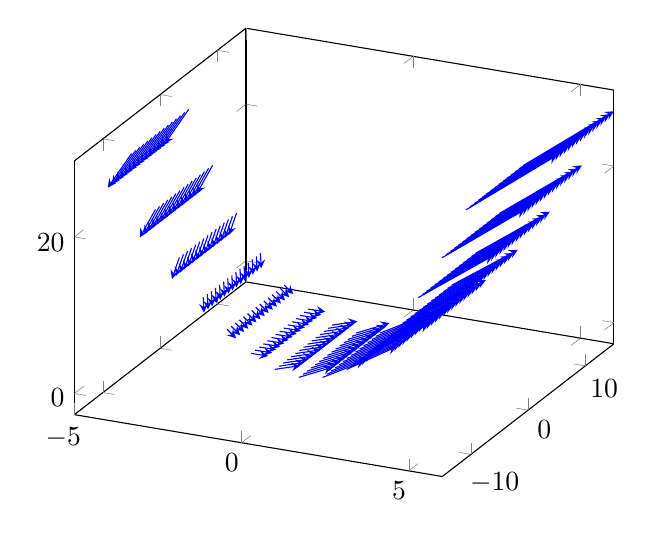
\begin{tikzpicture}
	\begin{axis}
		\addplot3[blue,
quiver={u=1,v=2*x,w=2},
-stealth,samples=15] {x^2};
	\end{axis}
\end{tikzpicture}
\end{frame}


\section{Resultate}

\subsection{Aggregatzustände} %vllt?



\subsection{Noch Mögliches} %Steht erstmal irgendetwas %TODO

\begin{frame}
  \frametitle{Welt}
    \vspace*{-0.3cm}
  \begin{block}{Objekte}
    \begin{itemize} 
      \item unpassierbare Objekte in den Raum platzieren
      \item permeable/semipermeable Objekte
    \end{itemize}
  \end{block}
    \pause
  \begin{block}{Observablen}
    \begin{itemize} 
      \item unterschiedliche Startgeschwindigkeiten
      \item v binomial auf die Teilchen verteilen
      \item abkühlen des Systems über Zeit
    \end{itemize}
  \end{block}
\end{frame}

\begin{frame}
    \vspace*{0.9cm}
    \centering
    \Huge
    Vielen Dank\\
    für\\
    Eure Aufmerksamkeit.\\
\end{frame}

\end{document}